% PWT Data Analysis
% Collects the exhibits produced by Honduras Excercises/do/02b_PWT_data_analysis.do.
% Build:  pdflatex "PWT Data Analysis.tex"  (run twice for the table of contents)
% Paths are relative to Honduras Excercises/reports/.

\documentclass[11pt]{article}

\usepackage[utf8]{inputenc}
\usepackage[T1]{fontenc}
\usepackage{lmodern}
\usepackage[margin=1in]{geometry}
\usepackage{graphicx}
\usepackage{booktabs}
\usepackage{longtable}
\usepackage{caption}
\usepackage[section]{placeins}
\usepackage{float}
\usepackage{hyperref}

\graphicspath{{../output/figures/}}

% Wrap a self-contained esttab tabular into a captioned float, shrunk to
% \textwidth only if it would otherwise be too wide.
\newsavebox{\statsbox}
\newcommand{\statstable}[3]{% #1 = tabular file, #2 = caption, #3 = label
  \begin{table}[htbp]\centering
  \caption{#2}\label{#3}%
  \sbox{\statsbox}{\input{#1}}%
  \resizebox{\ifdim\wd\statsbox>\textwidth\textwidth\else\wd\statsbox\fi}{!}{\usebox{\statsbox}}%
  \end{table}}

\title{PWT Data Analysis}
\author{Samuel Su\'arez}
\date{\today}

\begin{document}
\maketitle
\tableofcontents
\bigskip

\noindent This report collects the descriptive output produced by
\texttt{02b\_PWT\_data\_analysis.do} (in \texttt{Honduras Excercises/do/}):
summary statistics for the key per-capita variables, a comparison of Honduras
against regional yearly averages, and a country-level data-availability table.
All monetary series are real --- GDP, capital and remittances per capita in
constant 2021 USD, the minimum wage in constant 2021 PPP USD; the
employment-to-population ratio and the Penn World Table human-capital index are
unitless.

\section{Summary statistics}

Tables~\ref{tab:sumstats-hnd}--\ref{tab:sumstats-wld} report, for each sample,
the number of country--year observations, the mean, standard deviation, minimum,
median and maximum of every variable. The samples are nested: Honduras
$\subset$ Central America \& the Caribbean $\subset$ Latin America $\subset$
World. $N$ is variable-specific (pairwise): human capital, remittances and the
minimum wage are observed for far fewer country--years than GDP.

\statstable{../output/tables/summary_stats_hnd.tex}{Summary statistics --- Honduras}{tab:sumstats-hnd}
\statstable{../output/tables/summary_stats_cac.tex}{Summary statistics --- Central America \& the Caribbean}{tab:sumstats-cac}
\statstable{../output/tables/summary_stats_lac.tex}{Summary statistics --- Latin America}{tab:sumstats-lac}
\statstable{../output/tables/summary_stats_wld.tex}{Summary statistics --- World (full PWT panel)}{tab:sumstats-wld}

\FloatBarrier
\section{Comparison of averages}

Each figure plots Honduras (thick cranberry line) against the yearly
cross-country mean of Central America \& the Caribbean, South America, Latin
America and the World. The dashed vertical line marks the 2009 coup. South
America contributes no remittances series (no CEPAL coverage).

\begin{figure}[htbp]
\centering
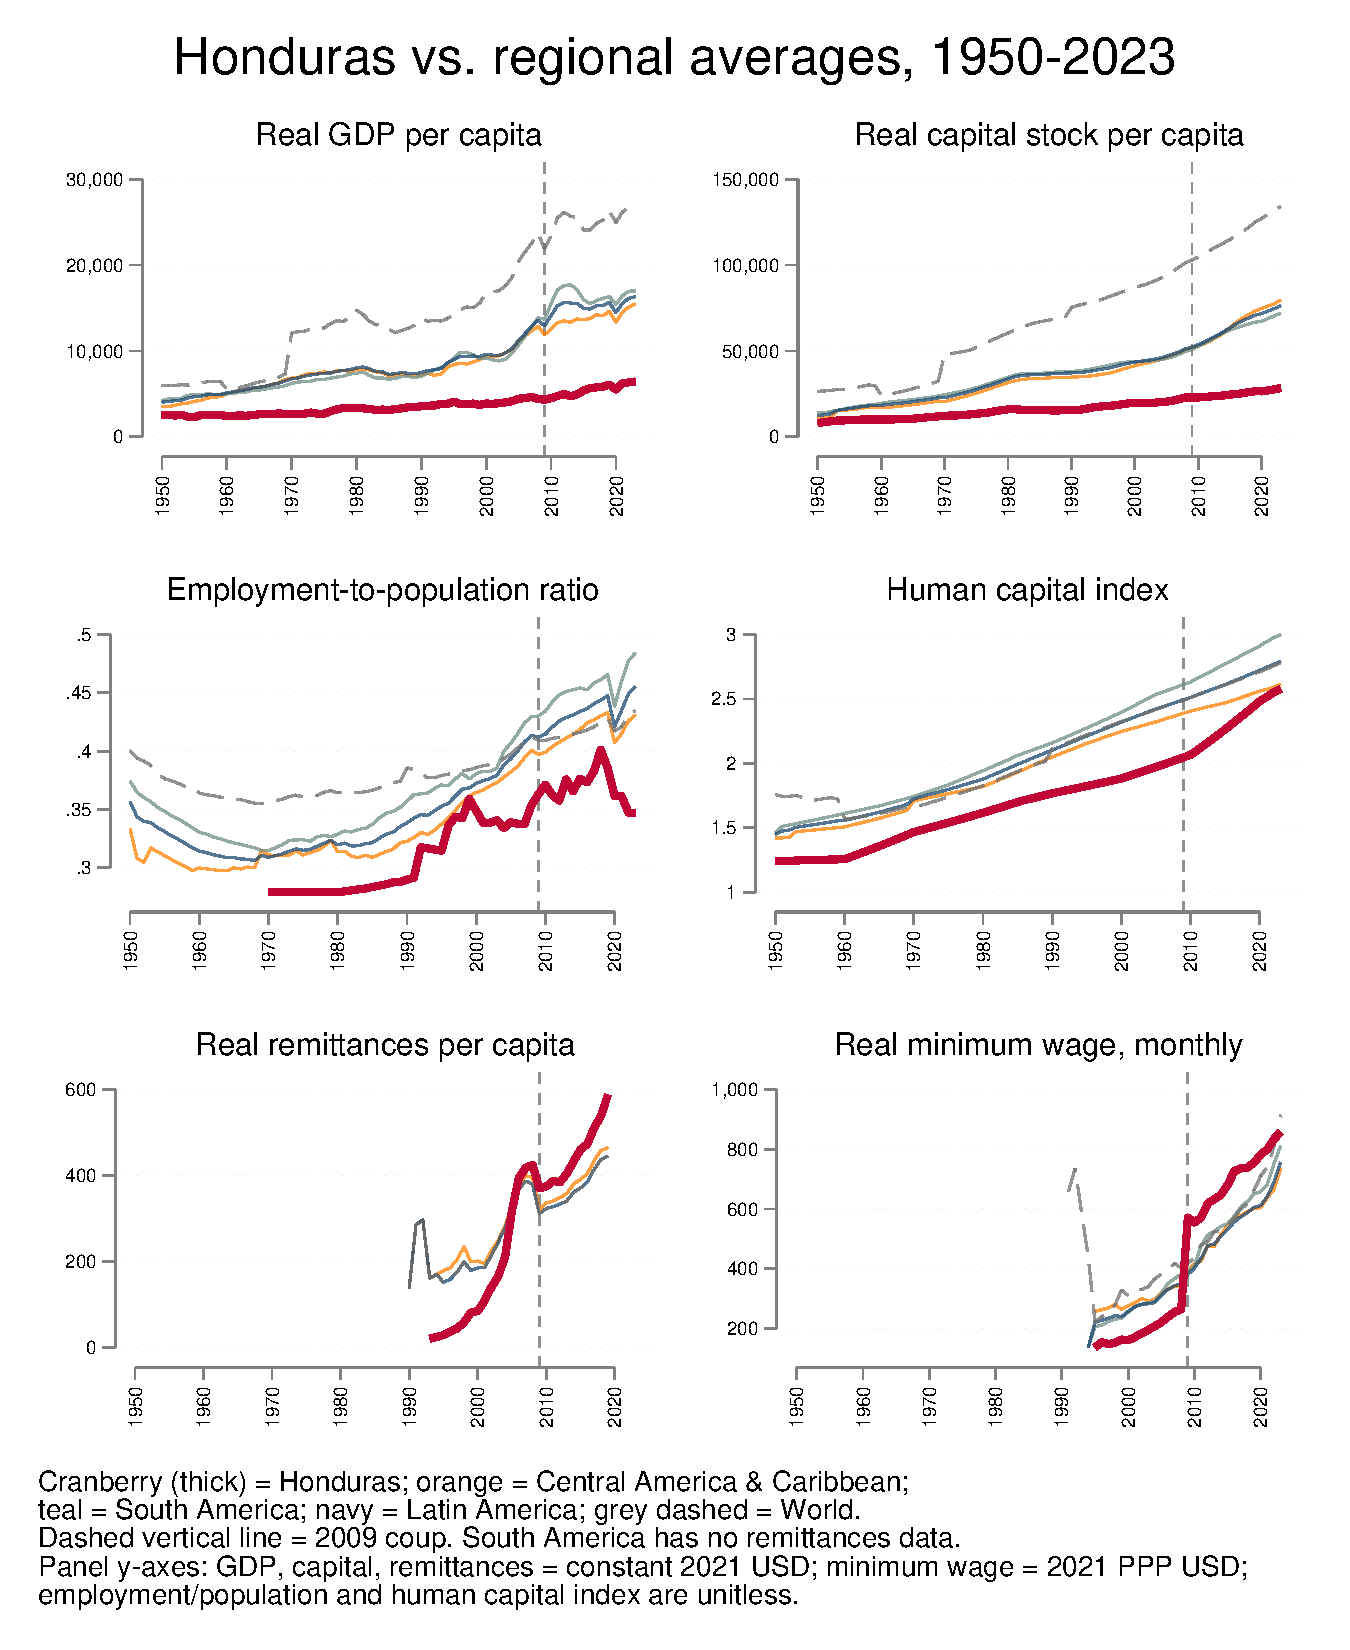
\includegraphics[width=0.92\linewidth]{avg_combined}
\caption{All variables: Honduras vs.\ regional yearly averages (overview grid).}
\label{fig:avg-combined}
\end{figure}

\begin{figure}[htbp]
\centering
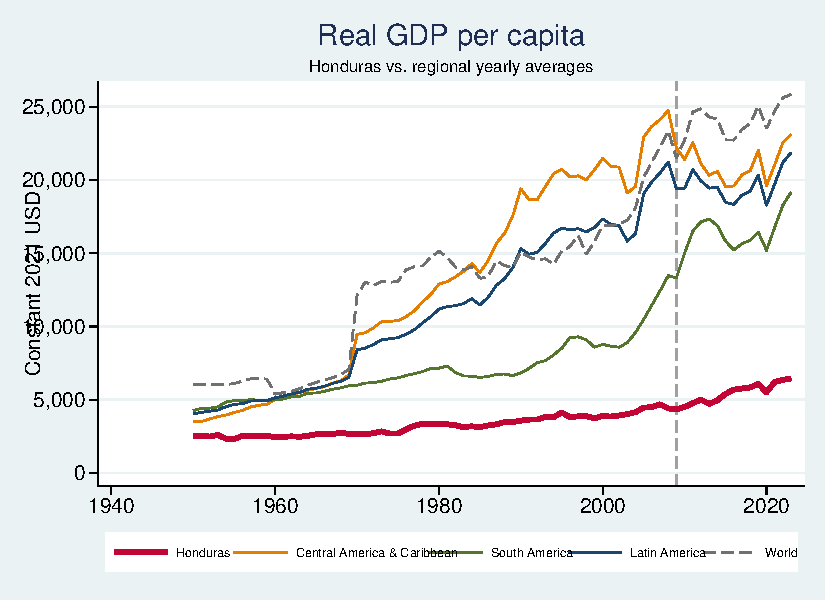
\includegraphics[width=0.82\linewidth]{avg_rgdpo_pc}
\caption{Real GDP per capita (constant 2021 USD): Honduras vs.\ regional averages.}
\label{fig:avg-rgdpo}
\end{figure}

\begin{figure}[htbp]
\centering
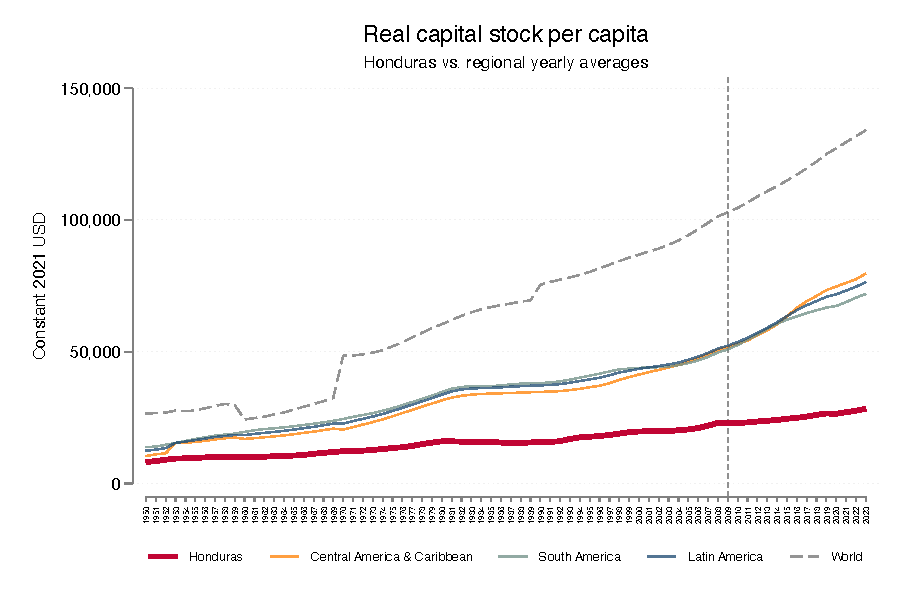
\includegraphics[width=0.82\linewidth]{avg_cap_pc}
\caption{Real capital stock per capita (constant 2021 USD): Honduras vs.\ regional averages.}
\label{fig:avg-cap}
\end{figure}

\begin{figure}[htbp]
\centering
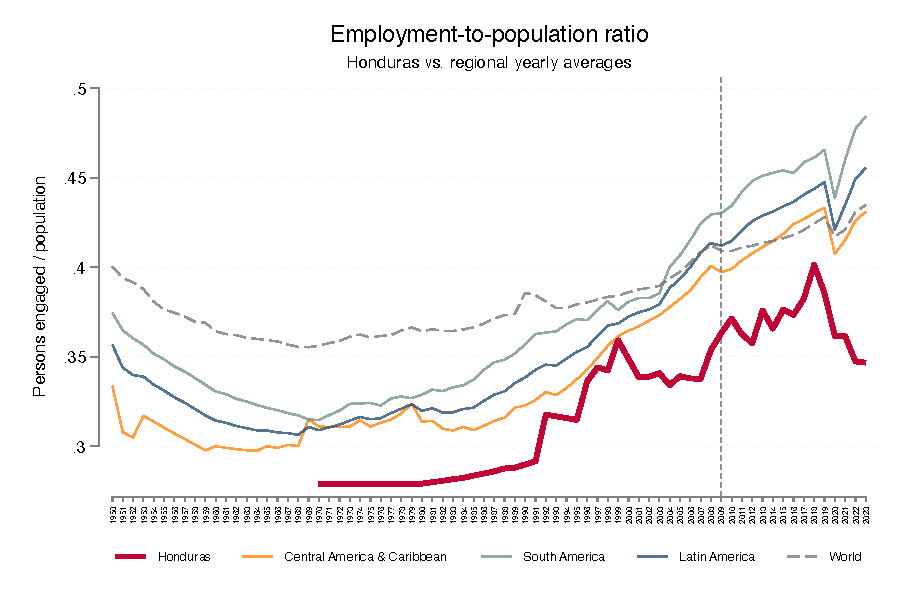
\includegraphics[width=0.82\linewidth]{avg_lab_pc}
\caption{Employment-to-population ratio: Honduras vs.\ regional averages.}
\label{fig:avg-lab}
\end{figure}

\begin{figure}[htbp]
\centering
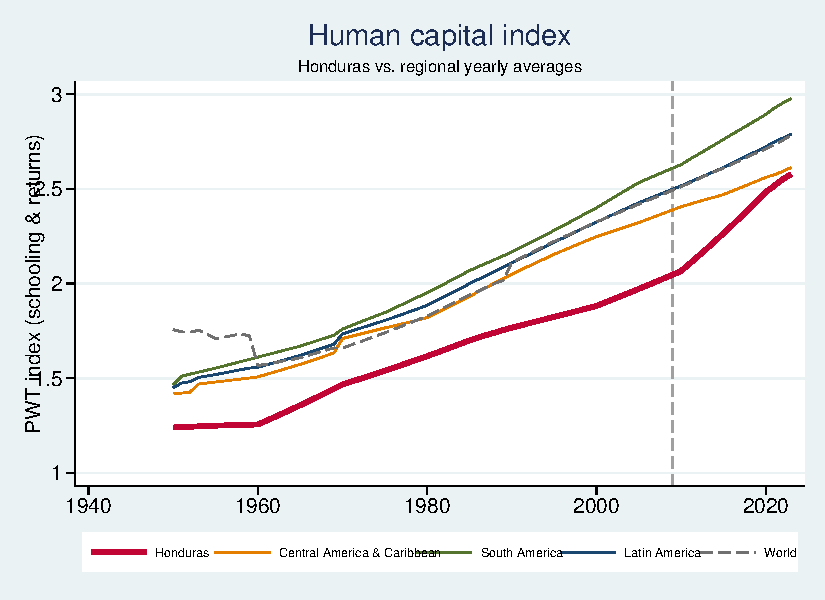
\includegraphics[width=0.82\linewidth]{avg_hc}
\caption{Human capital index (Penn World Table): Honduras vs.\ regional averages.}
\label{fig:avg-hc}
\end{figure}

\begin{figure}[htbp]
\centering
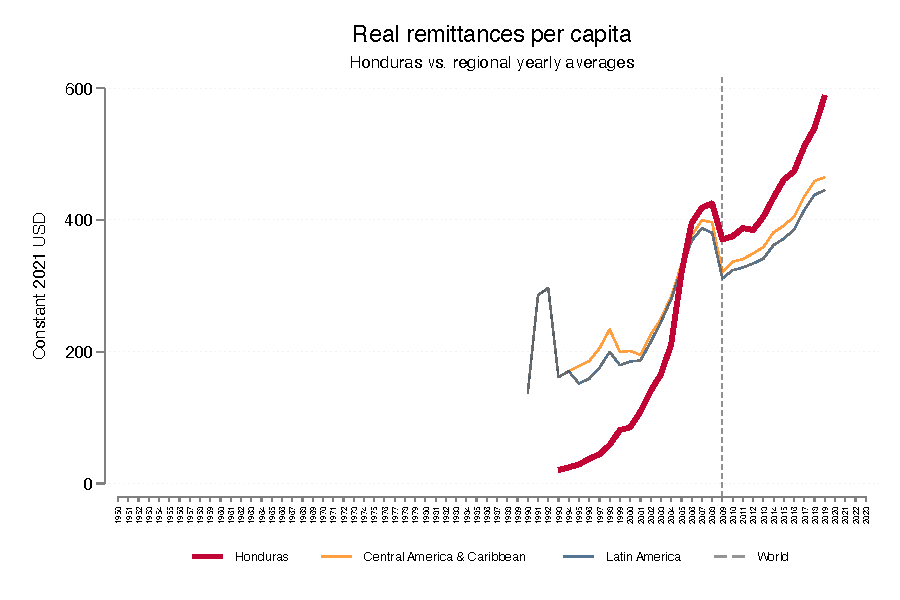
\includegraphics[width=0.82\linewidth]{avg_remittances_real_pc}
\caption{Real remittances per capita (constant 2021 USD): Honduras vs.\ regional averages.}
\label{fig:avg-remit}
\end{figure}

\begin{figure}[htbp]
\centering
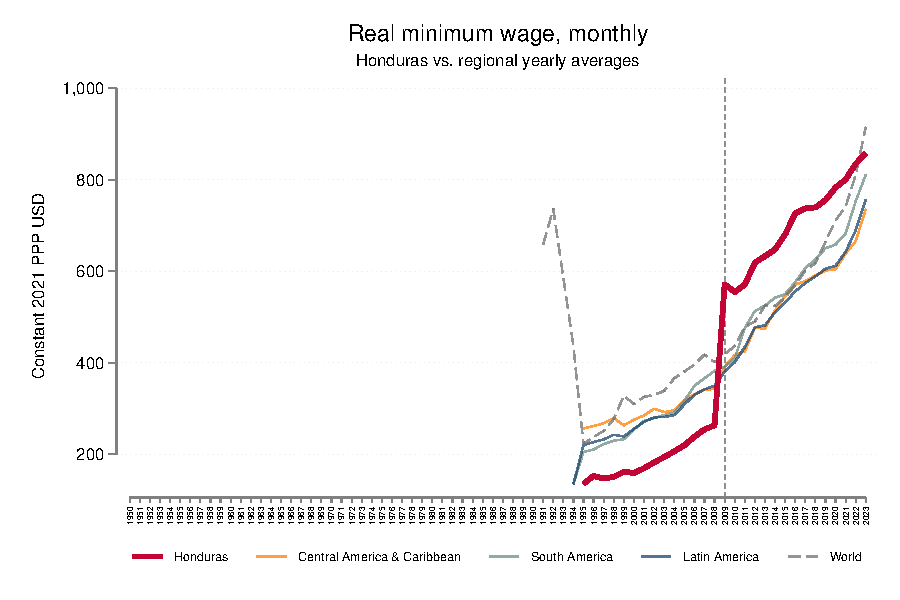
\includegraphics[width=0.82\linewidth]{avg_minwage_ppp}
\caption{Real minimum wage, monthly (constant 2021 PPP USD): Honduras vs.\ regional averages.}
\label{fig:avg-minwage}
\end{figure}

\FloatBarrier
\section{Data availability by country}

Table~\ref{tab:coverage} lists, for every Penn World Table country, the span of
years each variable is observed: \texttt{first--last}, a lone year if only one
is present, a trailing \texttt{*} if the span has internal gaps, and
\texttt{.}\ if the variable is never observed. Remittances are available only for
the eight CEPAL countries; the minimum wage is the ILO ``2021 PPP \$'' slice.

\begingroup
\scriptsize
\setlength{\tabcolsep}{3pt}
\input{../output/tables/data_coverage.tex}
\endgroup

\FloatBarrier
\section{SCM-eligible countries by donor pool}

Section~\ref{sec:scm-countries} lists, for each donor pool used by
\texttt{03b\_PWT\_SCM\_implementation.do}, the countries that remain after
requiring complete real GDP, capital stock, employment and human-capital data
over 1993--2019 (see \texttt{01b\_PWT\_data\_cleaning.do}, section~5) --
countries with even a single missing year in any of these four abort any
synth model that touches it.
\label{sec:scm-countries}

% SCM-eligible countries by donor pool -- 02b sec.5
\begin{description}
\item[World (144)] Albania, Algeria, Angola, Argentina, Armenia, Australia, Austria, Bahrain, Bangladesh, Barbados, Belgium, Belize, Benin, Bolivia (Plurinational State of), Botswana, Brazil, Brunei Darussalam, Bulgaria, Burkina Faso, Burundi, Cambodia, Cameroon, Canada, Central African Republic, Chile, China, China, Hong Kong SAR, China, Macao SAR, Colombia, Congo, Costa Rica, Croatia, Cyprus, Czechia, Côte d'Ivoire, D.R. of the Congo, Denmark, Dominican Republic, Ecuador, Egypt, El Salvador, Estonia, Eswatini, Ethiopia, Fiji, Finland, France, Gabon, Gambia, Germany, Ghana, Greece, Guatemala, Haiti, Honduras, Hungary, Iceland, India, Indonesia, Iran (Islamic Republic of), Iraq, Ireland, Israel, Italy, Jamaica, Japan, Jordan, Kazakhstan, Kenya, Kuwait, Kyrgyzstan, Lao People's DR, Latvia, Lesotho, Liberia, Lithuania, Luxembourg, Madagascar, Malawi, Malaysia, Maldives, Mali, Malta, Mauritania, Mauritius, Mexico, Mongolia, Morocco, Mozambique, Myanmar, Namibia, Nepal, Netherlands, New Zealand, Nicaragua, Niger, Nigeria, Norway, Pakistan, Panama, Paraguay, Peru, Philippines, Poland, Portugal, Qatar, Republic of Korea, Republic of Moldova, Romania, Russian Federation, Rwanda, Saudi Arabia, Senegal, Serbia, Sierra Leone, Singapore, Slovakia, Slovenia, South Africa, Spain, Sri Lanka, Sudan, Sweden, Switzerland, Syrian Arab Republic, Taiwan, Tajikistan, Thailand, Togo, Trinidad and Tobago, Tunisia, Türkiye, U.R. of Tanzania: Mainland, Uganda, Ukraine, United Arab Emirates, United Kingdom, United States, Uruguay, Venezuela (Bolivarian Republic of), Viet Nam, Yemen, Zambia, Zimbabwe
\item[Latin America (23)] Argentina, Barbados, Belize, Bolivia (Plurinational State of), Brazil, Chile, Colombia, Costa Rica, Dominican Republic, Ecuador, El Salvador, Guatemala, Haiti, Honduras, Jamaica, Mexico, Nicaragua, Panama, Paraguay, Peru, Trinidad and Tobago, Uruguay, Venezuela (Bolivarian Republic of)
\item[South America (10)] Argentina, Bolivia (Plurinational State of), Brazil, Chile, Colombia, Ecuador, Paraguay, Peru, Uruguay, Venezuela (Bolivarian Republic of)
\item[Central America \& the Caribbean (12)] Barbados, Belize, Costa Rica, Dominican Republic, El Salvador, Guatemala, Haiti, Honduras, Jamaica, Nicaragua, Panama, Trinidad and Tobago
\end{description}


\FloatBarrier
\section{Aprendizajes (ejercicios de Cunningham)}

Notas tomadas de \texttt{Cunningham Excercises/Texas\_Prisons/Do/Script.do}
(m\'etodo de control sint\'etico, r\'eplica de Texas), que orientan las
preguntas abiertas de \texttt{questions.txt}.

\subsection*{Sobre predictores y \emph{matching}}
\begin{quote}
\noindent Aprendizajes: \\
1) Es útil ver para honduras gdp\_mean vs gdp\_honduras. Los años donde honduras
se desvíe pueden ser usados como regresores como proxy de los no observados.
Esto es como decirle al modelo: Considera que honduras se desvio en t año y por
lo tanto debes darle un peso distinto a los paises que tomen en cuenta ese año. \\
2) Lo mismo se puede hacer con otros regresores. \\
3) La combinación de distintos periodos de la variable a predecir \\
4) Dejar una covariable sola (sin el año) hace que se tome un promedio de su
valor en todos los años en el matching discrepancy. \\
5) Si los pesos se hacen con las x, esto implica que estamos asumiendo que
Y es una función lineal de las x. DUDA $\to$ Entonces como se hace con ML?
\end{quote}

\subsection*{Sobre el tama\~no del \emph{donor pool} y los p-valores}
\begin{quote}
\noindent Aprendizajes: \\
Con todos los países de centro américa no basta para tener signif. estadíst. \\
El mejor p-valor posible es 1/7 = 0.143. \\
Para un p-valor de 0.1, se necesitan 10 países. \\
Para un p-valor de 0.05, se necesitan 20 países. $\to$ America Latina basta \\
Para un p-valor de 0.01, se necesitan 100 países. $\to$ El sur global tiene 173
\end{quote}

\end{document}
